\subsection{Analys} \label{sec:analysis}

\subsubsection{Detektorns känslighet} \label{sec:sensitivity}

I figur~\ref{fig:sensitivityraw} visas uppmätta värden på detektorns
känslighet \parencite{instructions}. Mätningarna har utförts genom ett
kalibreringsprov vars aktivitet är känt. Figuren visar mätdatapunkter
och en anpassad kurva.

\begin{figure}[!hp]
    \centering
    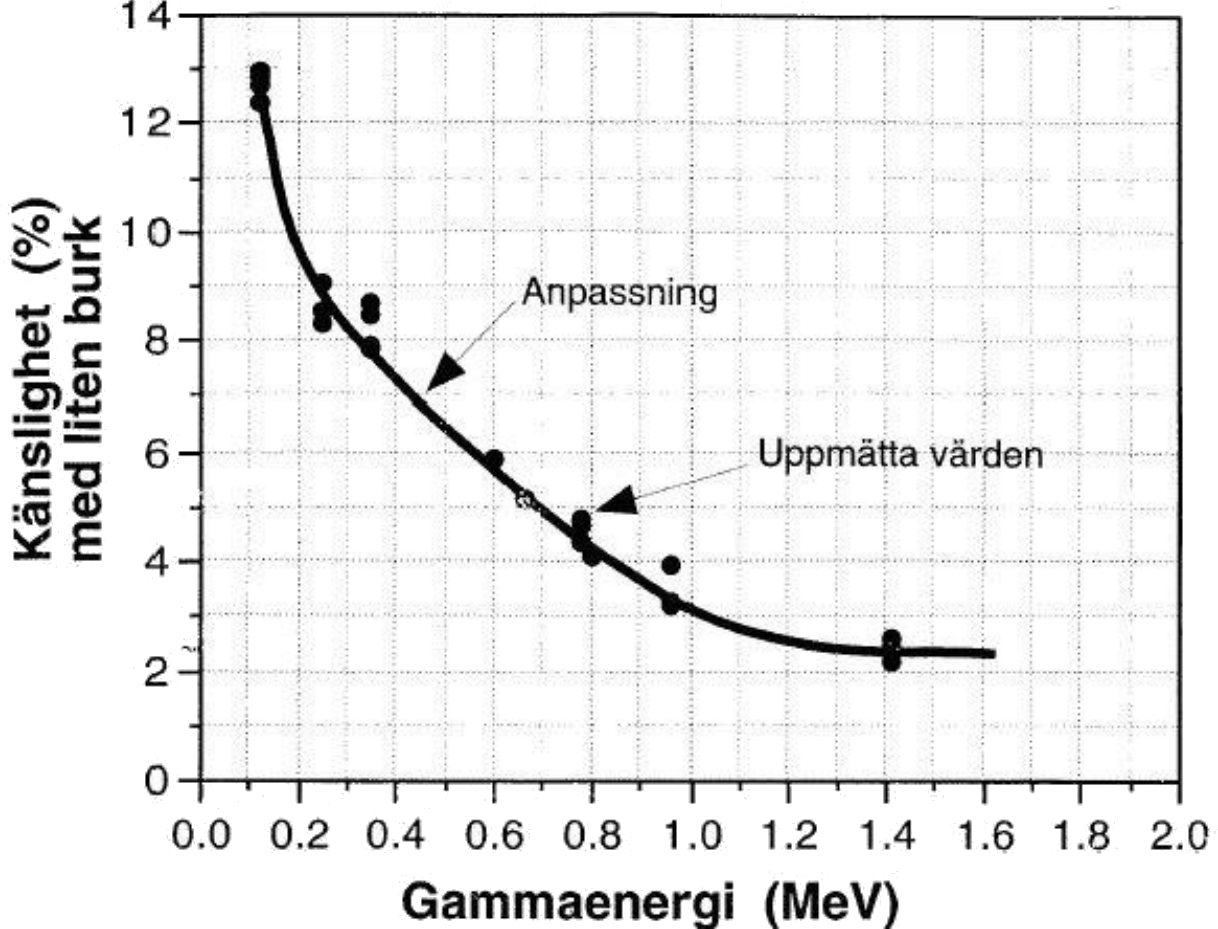
\includegraphics[width=\textwidth, keepaspectratio]{../images/sensitivity_raw.png}
    \caption{
        Detektorns känslighet vid olika energinivåer beräknad genom
        kalibreringsprov, men mätdatapunkter och anpassningskurva.
    }
    \label{fig:sensitivityraw}
\end{figure}

Då varken kurvans funktion eller mätvärdena är givna kan inga exakta värden
avläsas. Dock visas i avsnitt~\ref{sec:measurements} att topparna i de båda
gammaspektrumen har relativt låg fördelning. Av denna anledning har funktionen
approximerats linjärt i utvalda intervall. För svampprovet, vars topp ligger i
intervallet \qtyrange{0.58}{0.75}{\MeV}, har linjen passats till punkterna
\point{0.60}{5.6} och \point{0.70}{5.0}. För saltprovet, vars topp ligger i
intervallet \qtyrange{1.38}{1.54}{\MeV}, har den passats till \point{1.40}{2.4}
och \point{1.55}{2.4}. Två värdesiffror har valts då ingen högre precision kan
utläsas av enbart bilden. Notera att den vertikala axeln i
figur~\ref{fig:sensitivityraw} anges i~\unit{\percent}. Linjerna $L_1$
respektive $L_2$ fås då av energin $E$ enligt:
%
\begin{align}
    L_1 &= \num{-0.060} E + \num{0.092} \label{eq:line1} \\
    L_2 &= \num{0.024}                 \label{eq:line2}
\end{align}
%
Dessa punkter, samt linjerna de ger upphov till, visas tillsammans med
anpassningen i figur~\ref{fig:sensitivity}.

\begin{figure}[!hp]
    \centering
    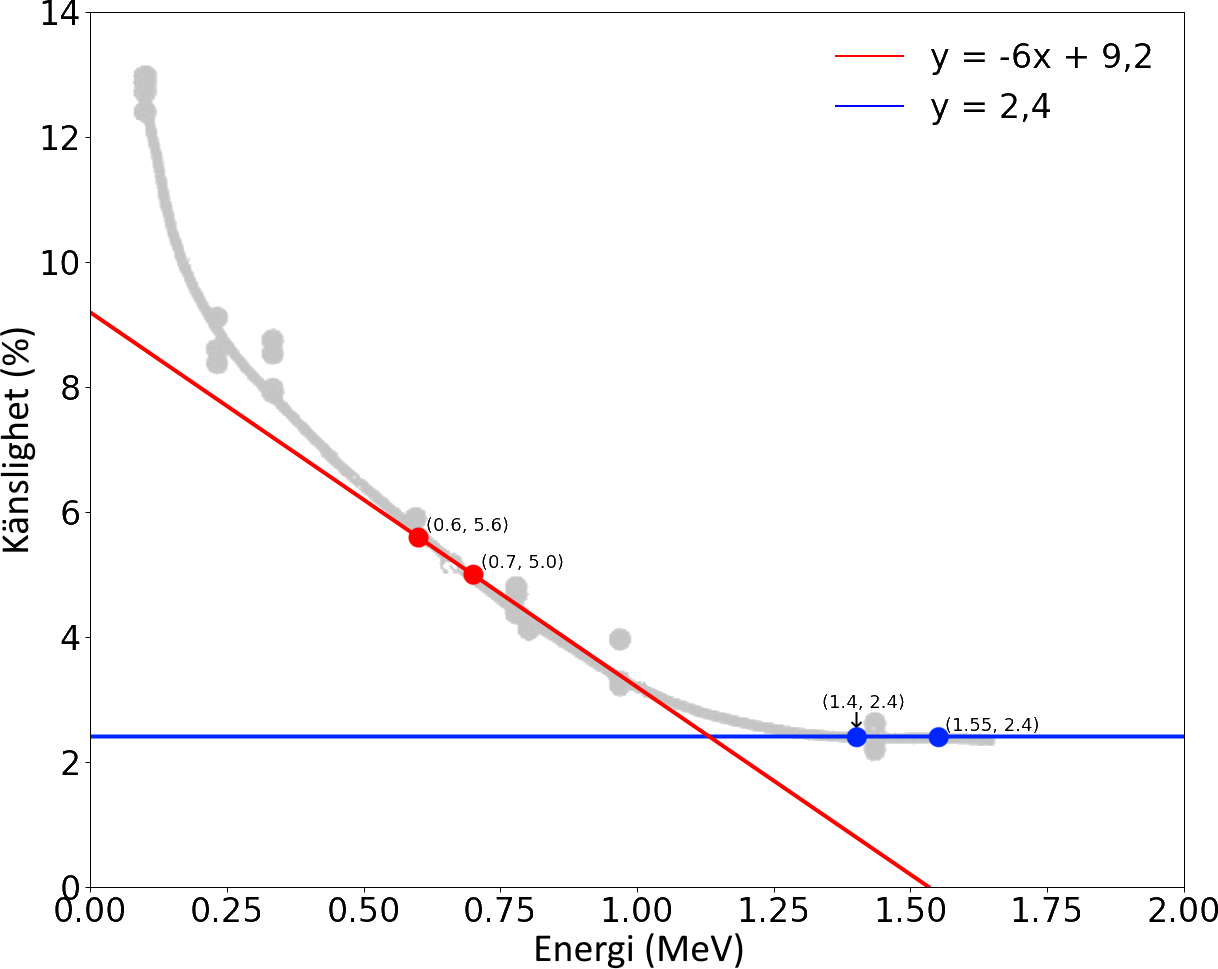
\includegraphics[width=\textwidth, keepaspectratio]{../images/sensitivity.png}
    \caption{
        Linjära uppskattningar av utvalda intervall av funktionen i
        figur~\ref{fig:sensitivityraw}. Pivotpunkter är markerade och linjernas
        funktioner anges (notera att dessa ges i~\unit{\percent}).
    }
    \label{fig:sensitivity}
\end{figure}

\subsubsection{Aktivitet i gammaspektrumen} \label{sec:activity}

Aktiviteten i proverna ska bestämmas. Denna kan dock inte utläsas direkt av
datan då detektorn i avsnitt~\ref{sec:sensitivity} visades ha en känslighet
på endast några \unit{\percent}, samt att inte nödvändigtvis alla södnerfall är
$\gamma$-sönderfall.

Låt $A$ vara den totala aktiviteten, $D$ sannolikheten att en atom
sönderfaller genom $\gamma$-sönderfall och $k$ känsligheten för någon given
energinivå $E_0$. Det fås att
%
\begin{equation}
    D = \frac{A_\gamma}{A} \label{eq:sharegamma},
\end{equation}
%
där $A_\gamma$ är antalet $\gamma$-sönderfall per sekund. Vidare fås att
%
\begin{equation}
    k = \frac{f}{A_\gamma} \label{eq:sensitivity},
\end{equation}
%
där $f$ är antalet uppmätta pulser vid $E_0$.

$D$ är för en given isotop en känd konstant, $f$ bestämdes experimentellt
i avsnitt~\ref{sec:measurements} och $k$ bestämdes som en funktion av
energinivån $E$ i avsnitt~\ref{sec:sensitivity}. Då $k$ inte är konstant, men
$f$ är bestämd för några diskreta energinivåer, skrivs \eqref{eq:sensitivity}
som en summa;
%
\begin{equation}
    A_\gamma = \sum_i \frac{f(E_i)}{k(E_i)} \inlineunit{\becquerel} \quad \text{\parencite{instructions}} \label{eq:sensitivitysum}.
\end{equation}
%
Genom insättning av \eqref{eq:sharegamma} i \eqref{eq:sensitivitysum} fås
%
\begin{equation}
    A = \frac{1}{D} \sum_i \frac{f(E_i)}{k(E_i)} \inlineunit{\becquerel} \quad \text{\parencite{instructions}} \label{eq:activitysum}.
\end{equation}

Givet aktiviteten kan provets aktivitet per massa $a$ (då massan är känd)
bestämmas enligt
%
\begin{equation}
    a = \frac{A}{m} \inlineunit{\becquerel\per\kg} \quad \text{\parencite{instructions}} \label{eq:apm}.
\end{equation}

Eftersom
%
\begin{align}
    A       &= \lambda N             &\quad \fysika{Fd2b} \label{eq:activity}, \\
    T_{1/2} &= \frac{\ln 2}{\lambda} &\quad \fysika{Fd2b} \label{eq:halflife},
\end{align}
%
kan även antalet atomer av den instabila nukliden $N$ bestämmas enligt
%
\begin{equation}
    N = \frac{A T_{1/2}}{\ln 2} \label{eq:substance}.
\end{equation}

För Cs-137 är $T_{1/2} = \qty{30.08}{\scyear}$ \fysika{Tk4},
$D = \num{0.851}$ \parencite{instructions} och för provet $m = \qty{18.0}{\g}$
(se avsnitt~\ref{sec:measurements}). Energinivåerna är i intervallet vars
känslighet uppskattas av \eqref{eq:line1}. Detta ger en aktivitet per massa
$a_{Cs} \approx \qty{1.8e4}{\becquerel\per\kg}$ och en substansmängd
$N_{Cs} \approx \num{4.4e11}$.

För K-40 är motsvarande värden $T_{1/2} = \qty{1.248}{\giga\scyear}$
\fysika{Tk4}, $D = \num{0.1067}$ \parencite{instructions}, $m = \qty{70.0}{\g}$
(avsnitt~\ref{sec:measurements}). Energinivåerna är i intervallet vars
känslighet uppskattas av \eqref{eq:line2}. Detta ger en aktivitet per massa
$a_K \approx \qty{6.3e3}{\becquerel\per\kg}$ och en substansmängd
$N_K \approx \num{2.5e19}$.

\subsubsection{Maximal sönderfallsenergi i betaspektrumet} \label{sec:betamax}

Att experimentellt bestämma ett maximalt värde för elektronenergin vid
det vanligaste $\beta$-sönderfallet är icke-triviellt; Cs-137 sönderfaller på
olika sätt (se avsnitt~\ref{sec:theory}). Detta innebär att spektrumet inte
visar energinivåer för en typ av reaktion utan överlappande nivåer för flera.
Analys av spetrumet måste oundvikligen kompensera för sannolikheter.

Den kontinuerliga fördelningen vid de lägre energinivåern utgör de sökta
sönderfallen; det vanligaste fallet beskrivet i \eqref{eq:csdecay2}.
Topparna mot högerkanten av spektrumet med något högre energinivåer motsvarar
sönderfallen i \eqref{eq:csdecay1}. De isolerade värdena utan klara
toppar som konstituerar övriga energinivåer beror dels på
bakgrundsstrålning, dels på sönderfallen genom inre konversion i
\eqref{eq:badecay2}.

Mätvärdena motiverar detta; energinivåer förbi den ``högra kanten'' nära
\qty{0.68}{\MeV} visar maximalt \num{2} pulser var, sammansatt \num{110}
stycken, av \num{1605} totala. Denna andel på \qty{6.8}{\percent} är kort
över den förväntade andelen \qty{5.6}{\percent} (\qty{1.5}{\percent}
felmarginal).

Ett antal möjliga metoder presenteras, med olika problem:
%
\begin{enumerate}
    \item Bestäm en Fermi-Kurie-plott och läs av det maximala värdet direkt.
    %
    \begin{itemize}
        \item De överlappande spektrumen beskrivna ovan gör det mycket svårt
        att bestämma en god och representativ sådan plott.
    \end{itemize}

    \item Beräkna teoretiskt ``perfekta'' fördelningar för de andra
    sönderfallen givet antal pulser, samt reaktionerna och deras sannolikheter.
    Subtrahera dessa spektrum från det uppmätta för att få ett där bara det
    vanligaste sönderfallet syns.
    %
    \begin{itemize}
        \item Då det uppmätta spektrumet är en relativt grov modell baserad på
        liten mängd mätdata och utrustning med icke-konstant känslighet för
        olika energinivåer innebär att det teoretiskt beräknade spektrumet inte
        helt skulle motsvara det uppmätta.

        \item Att vidare kompensera för känsligheten är svårt och går inte att
        göra med god precision av anledningar beskrivna i
        avsnitt~\ref{sec:sensitivity}.
    \end{itemize}

    \item Antag att sönderfallen i \eqref{eq:badecay2} är försumbara i
    intervallet som domineras av de i \eqref{eq:csdecay1} och
    \eqref{eq:csdecay2}. Välj vidare en punkt där spektrumet övergår från att
    domineras av \eqref{eq:csdecay2} till \eqref{eq:csdecay1}. Anpassa en kurva
    till det tidigare området och läs av minimipunkt.
    %
    \begin{itemize}
        \item Metoden baseras på ett antagande och en punkt som måste väljas
        genom manuell-visuell inspektion.

        \item Teorin föreslår linjär regression, men detektorns känslighet och
        empiriska resultat (exempelvis de bakom Fermi-Kurie-plottar) föreslår
        att kvadratisk regression kan vara bättre lämpad.
        Figur~\ref{fig:cesiumzoom} liknar en parabel mer än en linje, och i
        fallet att en linje trots det passar bättre kommer andragradskurvan
        reduceras till en linje.
    \end{itemize}
\end{enumerate}

Här har regression utförts. Vänsterkanten har valts till \qty{0.125}{\MeV} där
de lägsta energiniveråna registrerats. I avsnitt~\ref{sec:cesium} valdes
topparnas vänserkant nära \qty{0.605}{\MeV}. Under antagande att det finns en
punkt där den ena komposanten övergår till att dominera den andra är denna
punkt den kontinuerliga fördelningens högerkant. Anpassningskurvan visas i
figur~\ref{fig:cesiumcurve}, tillsammans med linjen där kurvan antar sitt
minimala värde. Kurvan beskrivs av
$y = \num{3943}x^2 - \num{4645}x + \num{1387}$ och antar sitt minsta värde i
$x \approx \qty{0.59}{\MeV}$. Detta värde är det beräknade värdet för den
maximala elektronenergin, och relativt nära det teoretiska värdet på
\qty{0.51}{\MeV} (se bilaga~\ref{sec:maxenergy}) (felmarginal
\qty{14}{\percent}).

\begin{figure}[!hp]
    \centering
    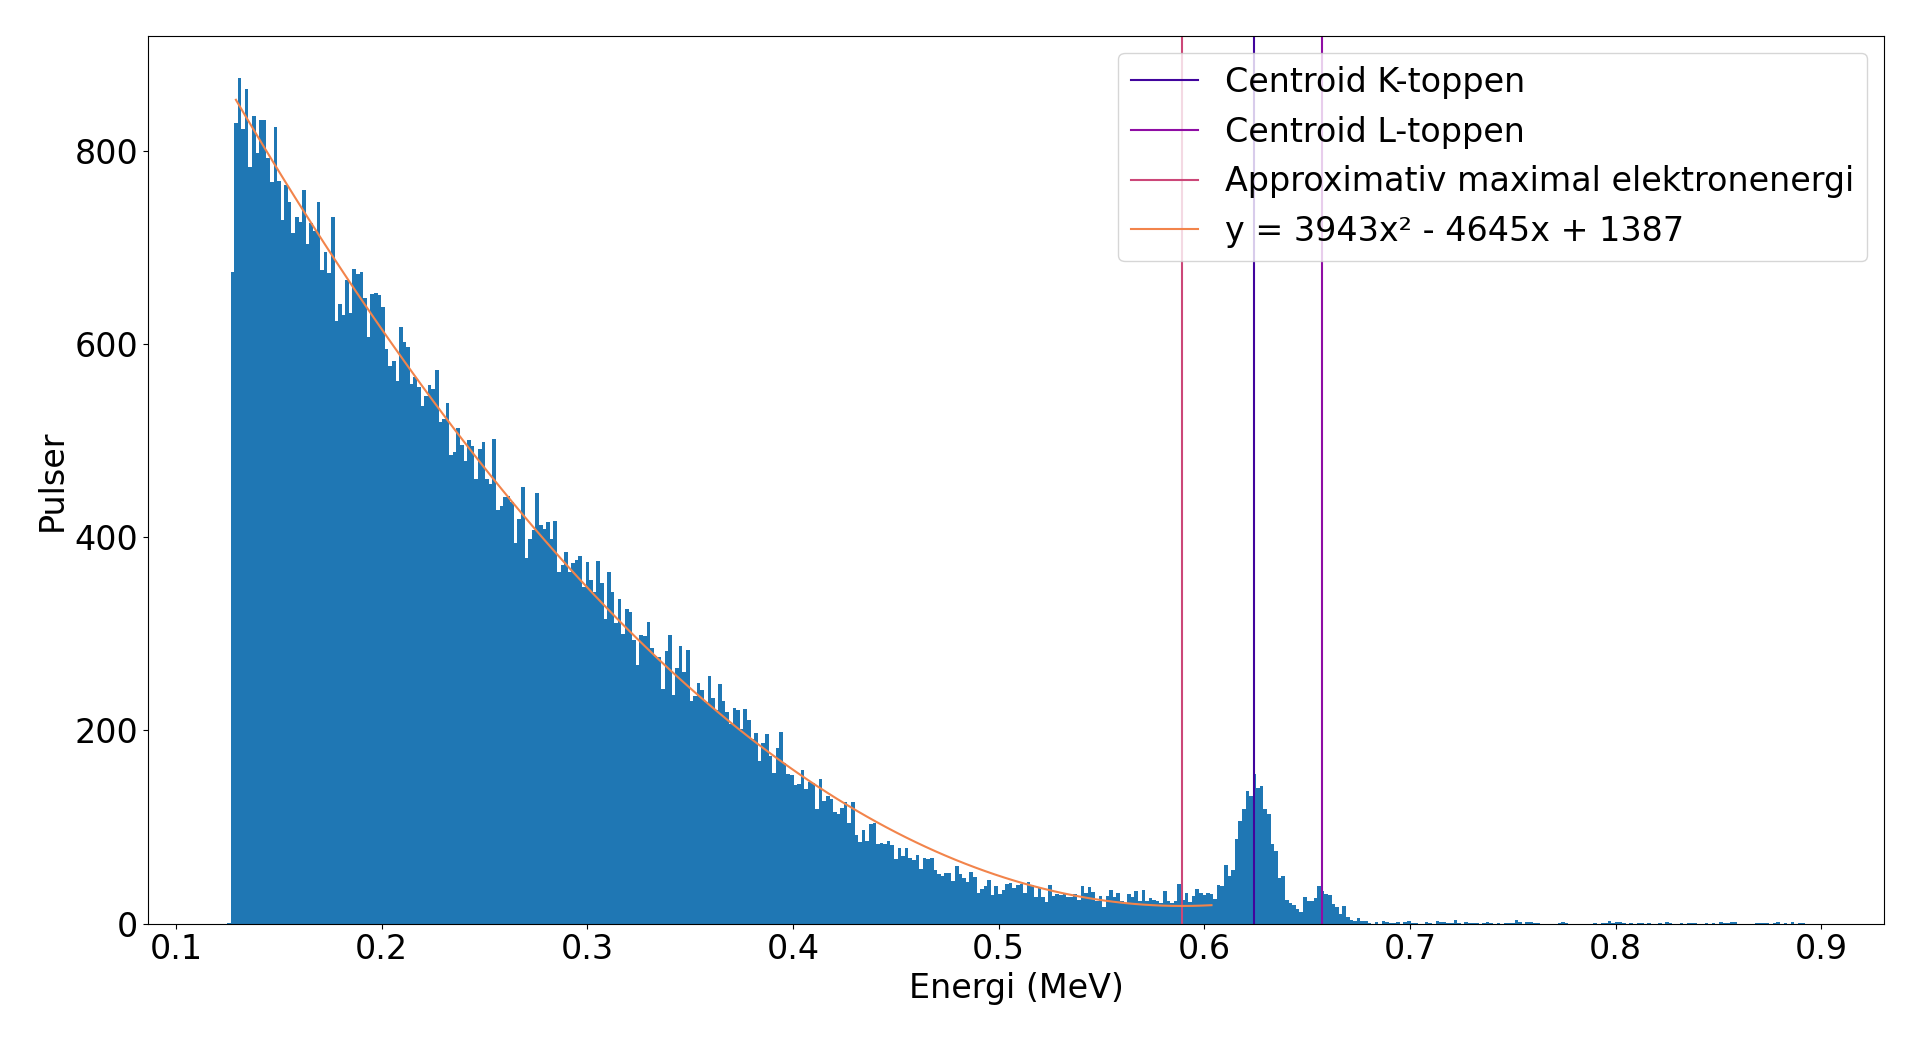
\includegraphics[width=\textwidth, keepaspectratio]{../images/cesium_curve.png}
    \caption{
        Betaspektrum från figur~\ref{fig:cesium} med kurvanpassning för
        kontinuerligt sönderfall. Kurvans funktion och minimipunkt är
        markerade.
    }
    \label{fig:cesiumcurve}
\end{figure}
